%%%%%%%%%%%%%%%%%%%%%%%%%%%%%%%%%%%%%%%%%%%%%%%%%%%%%%%%%%%%%%%%%%%%%%%%%%%%%%%%%%%%%%%%%%%%%%%%%%%%%%%%%%%%%%%%%%%%%%%%%%%%%%%%%%%%%%%%
% This is just a template to use when submitting manuscripts to Frontiers, it is not mandatory to use frontiers.cls nor frontiers.tex  %
%%%%%%%%%%%%%%%%%%%%%%%%%%%%%%%%%%%%%%%%%%%%%%%%%%%%%%%%%%%%%%%%%%%%%%%%%%%%%%%%%%%%%%%%%%%%%%%%%%%%%%%%%%%%%%%%%%%%%%%%%%%%%%%%%%%%%%%%

\documentclass{frontiersSCNS} % for Science articles
%\documentclass{frontiersMED} % for Medicine articles

\usepackage{url}
\usepackage{tabularx}
\usepackage{lineno}
\usepackage{multirow}
\usepackage[english]{babel}
\linenumbers


\copyrightyear{}
\pubyear{}
%\onecolumn
%%% write here for which journal %%%
\def\journal{Neurosciences}
\def\DOI{}
\def\articleType{}
\def\citing{\color{darkgray}\cite}
\def\keyFont{\fontsize{6}{11}\helveticabold }
\def\firstAuthorLast{Duda {et~al}} %use et al only if is more than 1 author
\def\Authors{Jeffrey T. Duda\,$^{1,*}$, Philip A. Cook\,$^{1}$ and James C. Gee\,$^1$}
% Affiliations should be keyed to the author's name with superscript numbers and be listed as follows: Laboratory, Institute, Department, Organization, City, State abbreviation (USA, Canada, Australia), and Country (without detailed address information such as city zip codes or street names).
% If one of the authors has a change of address, list the new address below the correspondence details using a superscript symbol and use the same symbol to indicate the author in the author list.
\def\Address{$^{1}$Penn Image Computing and Science Laboratory, University of Pennsylvania, Department of Radiology, Philadelphia, PA, USA}
% The Corresponding Author should be marked with an asterisk
% Provide the exact contact address (this time including street name and city zip code) and email of the corresponding author
\def\corrAuthor{Jeffrey T. Duda}
\def\corrAddress{Penn Image Computing and Science Laboratory, University of Pennsylvania, Department of Radiology, 3600 Market Street, Suite 370, Philadelphia, PA, USA}
\def\corrEmail{jtduda@seas.upenn.edu}

% \color{FrontiersBlue} Is the blue color, used in the Journal name, in the title, and the names of the sections


\begin{document}
\onecolumn
\firstpage{1}

\title[Reproducibility of structural graph metrics]{Reproducibility of graph metrics of human brain structural networks}
\author[\firstAuthorLast ]{\Authors}
\address{}
\correspondance{}
\editor{}
\topic{Neuroinformatics with the Insight ToolKit}

\maketitle
\begin{abstract}

%\section{}
%As a primary goal, the abstract should render the general significance and conceptual advance of the work clearly accessible to a broad readership. References should not be cited in the abstract.
%See the Summary Table at \\ \url{http://www.frontiersin.org/}\texttt{\journal}\url{/authorguidelines} \\for abstract requirement and length according to article type.
% Abstract Max Length = 2000 characters
Recent interest in human brain connectivity has led to the application of
graph theoretical analysis to human brain structural networks, in
particular white matter connectivity inferred from diffusion imaging
and fiber tractography. While these methods have been used to study a
variety of patient populations, there has been less examination of the
reproducibility of these methods. These graph metrics typically derive
from fiber tractography, however a number of tractography algorithms
exist and many of these are known to be sensitive to user-selected
parameters. The methods used to derive a connectivity matrix from
fiber tractography output may also influence the resulting graph
metrics. Here we examine how these algorithm and parameter choices
influence the reproducibility of proposed graph metrics on a publicly
available test-retest dataset consisting of 21 healthy young
adults. Network summary
measures are examined using the intraclass correlation coefficient
(ICC), and the dice coefficient is used to examine overlap 
of constant density subgraphs. 

%A freely available data set, the Multi-Modal MRI Reproducibility Resource, will serve as the basis for this study. ANTs, based upon ITKv4, will be used for the registration and segmentation steps needed to align and label individual brains. Camino, an open-source toolkit, will be used for: DT reconstruction, fiber tracking, and the generation of structural connectivity matrices. An ITK module will be created to implement the graph analysis metrics.


\tiny
  \section{Keywords:} Structure Tractography Connectivity Brain
  Network Reproducibility Graph  %All article types: you may provide up to 8 keywords; at least 5 are mandatory.
\end{abstract}

% For Technology Reports the introduction should be succinct, with no subheadings.
\section{Introduction}
Combining magnetic resonance imaging (MRI) of the human brain with graph
theory analysis has emerged as a powerful approach to studying
large-scale networks of both structural and functional
connectivity. In the case of structural connectivity, the use of diffusion weighted MRI and
associated fiber tractography methods provide the ability to identify
the long-range pathways that connect cortical regions and form a
network architecture~\citep{Basser2000,Lazar2003,Hagmann2003,Mori1999}. 
The use of graph theoretical analysis to study
the topology of these structural networks has increasingly been used to
examine the structural consequences of neurological disorders \citep{Xie2012,Basset2012}
as well as the relationship between structure and function \citep{}. 

Previous studies examining the reproducibly of graph-based metrics in
functional networks have shown good levels of reproducibly in MEG
\citep{Deuker2009}, fMRI using BOLD contrast
\citep{Telesford2010,Braun2012,Schwarz2011,Liang2012,Weber2013} and
arterial spin labeling \citep{Weber2013}. A number of studies have also examined
reproducibly in structural networks, each focusing on various aspects
of the complex processing pipeline that is a prerequisite for these
measures. These have included studies of diffusion spectrum imaging
\citep{Cammoun2012,Bassett2011N} and high angular resolution diffusion
imaging \citep{Dennis2012}. Some studies have examined probabilistic
tractography \citep{Owen2013BC,Vaessen2010}. DTI-based studies using
deterministic tractography have included the examination of
tractography seed density \citep{Cheng2012N}, anatomic label density
\citep{Bassett2011N}, and studies examining a variety of network
measures \citep{Cheng2012N,Irimia2012N}. In the paper we constrain our
analysis DTI-based deterministic fiber
tractography. Within this constraint, we examine multiple algorithms
for computing streamlines and their required parameters to examine
their influence on the final graph metrics. A set of manually defined
cortical parcellations \citep{Klein2012} is used along with a more common template-based
parcellation scheme \citep{AAL}. We use freely
available data and software to create a framework that facilitates future extensions
that may examine additional aspects of the processing as well as the
comparison to, or addition of, multiple imaging modalities. 

%Test retest of functional graph metrics via MEG \citep{Deuker2009}\\
%Test retest of functional graph metrics via fMRI \citep{Telesford2010,Liang2012,Braun2012}\\
%Test retest of structural graph metrics via DTI \citep{Owen2013BC}\\ 
%Test retest of structural graph metrics via DTI acquisition parameters \citep{Vaessen2010}\\
%Test retest of soft thresholding in fMRI \citep{Schwarz2011}\\
%Test restest of functional graph metrics via ASL \citep{Weber2013}\\
%Test retest of structural graph metrics via DTI and DSI with multiple labeling schemes \citep{Bassett2011N}\\
%Intra and inter subject variability of structural graph metrics via DTI for binary and weighted networks \citep{Cheng2012N}\\
%Correlations between pairs of regions using a variety of structural measures \citep{Irimia2012N}\\


%\textbf{Novel contributions}
%\begin{enumerate}
%\item Public data and fully open source
%\item In-depth examination of deterministic tractography parameters
%\item Probabilistic tractography extensions
%\item In-depth analysis of streamline-to-matrix conversion
%\item Provides plug-and-play framework for evaluation of new methods and/or alternate data sets
%\item Easy to extend to functional study (BOLD and ASL) 
%\end{enumerate}


%\begin{methods}
\section{Materials \& Methods}
% Materials and Methods: This section may be divided by subheadings. This section should contain sufficient detail so that when read in conjunction with cited references, all procedures can be repeated.

\subsection{Neuroimaging data}
The Multi-Modal MRI Reproducibility Resource~\citep{Landman2011}
provides a publicly available test-retest data set consisting of 21
healthy control subjects (11 males). The mean
age is 31.76 $\pm$ 9.35 with a range of [22,61]. This data set provides a
multitude of MR image types, but here only the T1-weighted anatomical images and diffusion
tensor images are examined.  The Mindboggle dataset provides a
population averaged template for this data set and for one time point
for each subject, a brain extracted image, and two sets of manually
defined cortical labels are provided \citep{Klein2012}.

\subsection{Anatomical data preprocessing}
ANTs volumetric-based cortical thickness estimation pipeline

The N4 tool was used to perform bias correction on each subject's T1
image \citep{Tustison????}. The antsRegistration tool was used to find
a deformable mapping between each subject's T1 and the Mindboggle
template for later use in anatomical labeling. An intra subject affine
registration was used to align each subject's T1 images. Thresholding
and a morphological closing was
used to obtain a brainmask from the brain extracted T1 images provided
by Mindboggle. 

For each subject, a set of manually defined cortical labels was
available via Mindboggle \citep{Klein2012}. Additionally, the AAL label set
\citep{Tzourio-Mazoyer2002} was also examined
as it is a label set often used in both functional and structural
studies. Here a template-based approach is used and the
antsRegistration tool is used to find a deformable mapping to the
Mindboggle template. These template mapping are then combined with the
intrasubject mapping to transfer the AAL labels into the DTI space for
each time point.

\subsection{Diffusion data preprocessing}
An affine registration was then used to align each T1
image to it's corresponding b=0 image that was acquired as part of the
DWI sequence. Composing these intrasubject mappings provides the
ability to transform labels between T1 and DTI space and between time
points for a subject.  The intra subject mappings
are then used to warp these labels into the DTI space for each time
point using nearest neighbor interpolation.

\subsection{Fiber tractography}
The Camino toolkit \citep{} is used to calculate diffusion tensor images via a
weighted linear fitting \citep{Basser1994,Salvador2005}, and is also
used to perform the deterministic tractography. The brainmasks defined
in anatomical space are warped into DTI space and are used to restrict the
tractography to eliminate false positives that could results from
streamlines that leave and then reenter the brain. Fractional anisotropy (FA) images are calculated and a
tractography seed-map is created by including all voxels with FA of at
least 0.2.

%These seed-maps are then resampled to a resolution of 0.5mm x 0.5mm x
%0.5mm to provide a dense seeding as this has been shown to increase stability of
%structural network metrics ~\citep{Cheng2012}. 

One of the primary differences among the various approaches to
deterministic tractograpy is the algorithm used to determine the
direction that a streamline should proceed from a given point. Here we
examine four different approaches:

\begin{enumerate}
\item Fiber Assignment by Continuous Tracking (FACT) - The primary
  direction of diffusion (PDD) is followed until the streamline enters
  a new voxel \citep{Mori1999}.
\item Euler -  The PDD is followed for a constant step size \citep{Basser2000}.
\item Rourth-order Runge-Kutta (RK4) - The direction of the step is determined
 by taking and averaging a weighted series of partial steps \citep{Basser2000}.
\item Tensor Deflection (TenD) - The entire diffusion tensor is used to deflect
the estimated fiber trajectory \citep{Lazar2003}
\end{enumerate}

%Additionally we examine the weighting parameters used in the TEND
%algorithm

\subsection{Graph generation}
For a given set of streamlines, the Camino toolkit is used to generate
a connectivity matrix that records how many streamlines connect each pair of
regions in a given set of labels. 

%Additionally, we generative matrices
%that record the average FA along all tracts that connect a given pair
%of regions. In both cases, the matrices may be thresholded for
%unweighted graph metrics or used as is for weighted graph metrics. 

\begin{table}[!t]
\processtable{Descriptions and references for graph metrics examined in this study.\label{tab:nodes}}
{\begin{tabular}{lll}
\midrule
Node metrics & Description & Reference\\\midrule
Degree & Number of connections for a node & \\
Clustering coefficient & Local neighborhood connectivity & \citep{Watts1998}\\
Path length & Average shortest path to all other nodes & \citep{Watts1998}\\
Global efficiency & ``Closeness'' to all other nodes & \citep{Latora2001}\\
Local efficiency & ``Closeness'' to local nodes & \\
\midrule
Whole-graph metrics\\
\midrule
Small-world & & \citep{Watts1998}\\
Synchronizability & & \citep{Motter2005}\\
Assortativity & & \citep{Newman2002}\\
Hierarchy & & \citep{Ravasz2003}\\
Cost efficiency & & \citep{Achard2007}\\
Rich-club coefficient & Degree to which high-degree nodes preferentially inter-connect & \citep{Colizza2006}\\
\midrule
Network similarity measures\\
\midrule
Network overlap & & \citep{vanWijk2010}\\
Edge overlap & Percentage of common edges in constant density networks & \citep{Weber2013} \\\botrule
\end{tabular}}{}
\end{table}

\subsection{Node metrics}
As we are interested in whole network summary measures, we examine the mean
over all nodes for each of the node-metrics listed in
table \label{tab:nodes}. For more details on the node metrics see
\citep{Rubinov2010}. An ITK module named Petiole was created to
calculate the desired network measures from the 2D connectivity
matrices \citep{Petiole}. This module incorporates and extends an existing implementation of a graph class \citep{NickITKJournal} and provides ITK functions for a variety of graph metrics while using the matlab-based Brain Connectivity Toolkit \citep{BCT} for algorithmic guidance. While many of these metrics inlude implementations for weighted graphs and directed graphs, here we focus on their application to unweighted, undirected graphs. 

\begin{table}[!t]
\processtable{Formulas for node metrics.\label{tab:equations}}
{\begin{tabular}{ll}
\midrule
Degree & $K_i = \sum_{j=1}^{n}{A_{ij}}$\\
Clustering coefficient & $C_i = 2*e_i / K_i ( K_i -1 )$\\
Path length & $L = 1/N(N-1) \sum_{ij \in n, i \neq j}{d_{ij}}$\\
Global efficiency & $E_{glob} = E(G) = 1/N(N-1) \sum_{i \neq j \in G}{1/d_{ij}}$\\
Local efficiency & $E_{loc} = 1/N \sum_{i \in n}{E(G_i)}$\\\botrule
\end{tabular}}{}
\end{table}

\subsection{Whole-graph metrics}
More formulas go here.

\subsection{Statistical analysis}
Dice coefficient for overlap of graph thresholded at a constant
density

$$Dice(x,y) = \frac{ 2 \| E(x) \cap E(y) \| }{ \|E(x) \| + \| E(y) |\ }$$
where $E(x)$ is the set of all edges in a graph, x, and edges are considered equal if they connect the same two nodes.

ICC was used to compare the

$$ICC = \frac{\sigma_{bs}^{2}}{\sigma_{bs}^{2} + \sigma_{ws}^{2}} $$

Permutation testing

%\textbf{Figure 1.}{ Enter the caption for your figure here.  Repeat as  necessary for each of your figures.}\label{fig:01}% Don't add the figures in the LaTeX files, please upload them when submitting the article. Frontiers will add the figures at the end of the provisional pdf.

%\end{methods}

\section{Results}
%Results: This section may be divided by subheadings. Footnotes should not be used and have to be transferred into the main text
Overview of what we found

\begin{figure}
\begin{center}
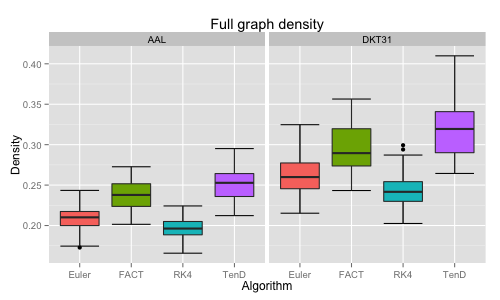
\includegraphics[width=0.5\linewidth]{figures/density_plot.png} 
\caption{Density}
\label{fig:density}
\end{center}
\end{figure}

\begin{figure}
\begin{center}
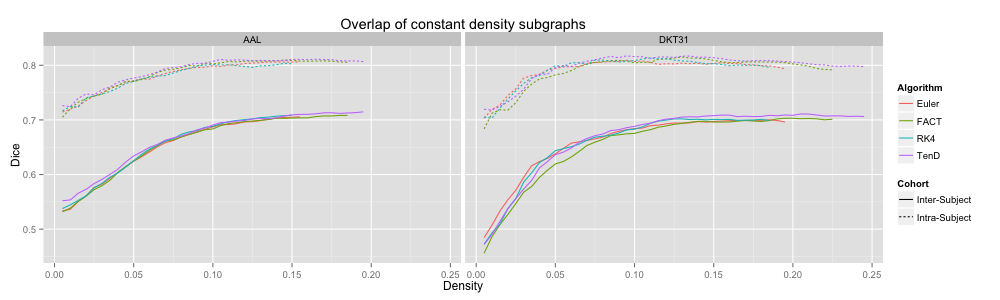
\includegraphics[width=0.5\linewidth]{figures/dice_overlap_plot.png} 
\caption{Dice}
\label{fig:dice}
\end{center}
\end{figure}

\begin{figure*}
\begin{center}
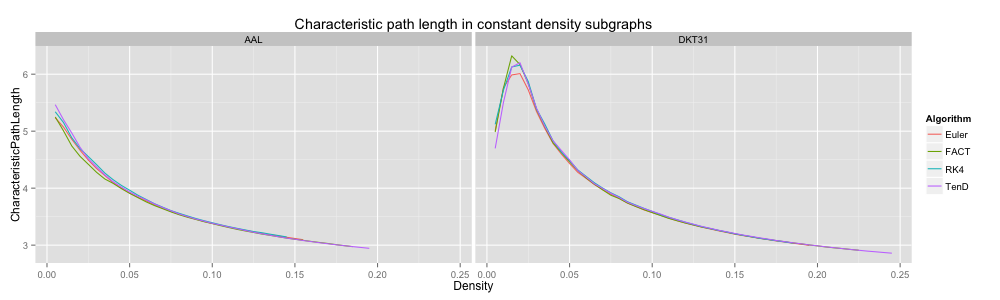
\includegraphics[width=\linewidth]{figures/path_plot.png} \\
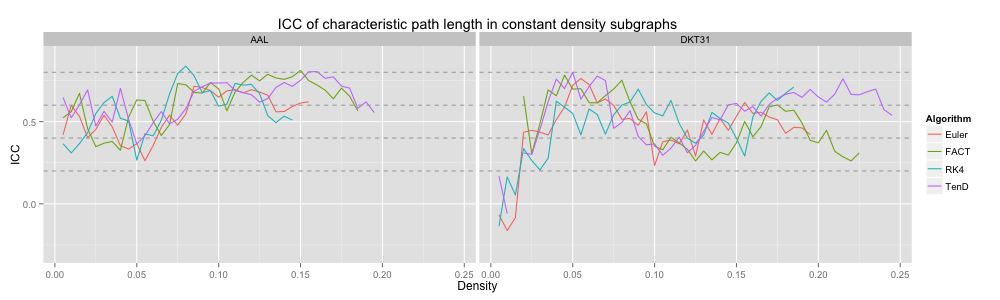
\includegraphics[width=\linewidth]{figures/path_icc_plot.png}
\caption{Path}
\label{fig:path}
\end{center}
\end{figure*}

\begin{figure*}
\begin{center}
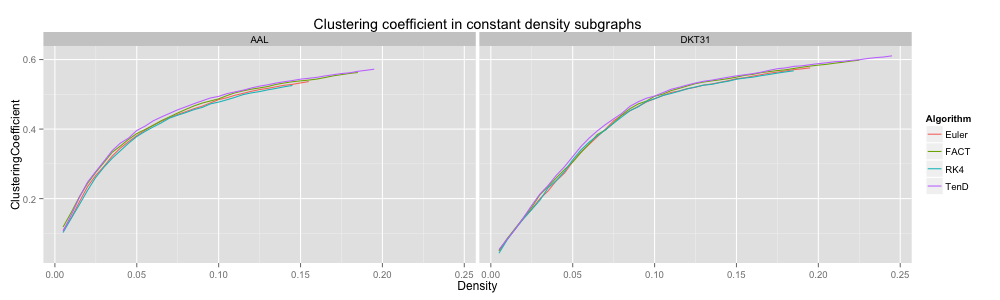
\includegraphics[width=\linewidth]{figures/clust_plot.png} \\
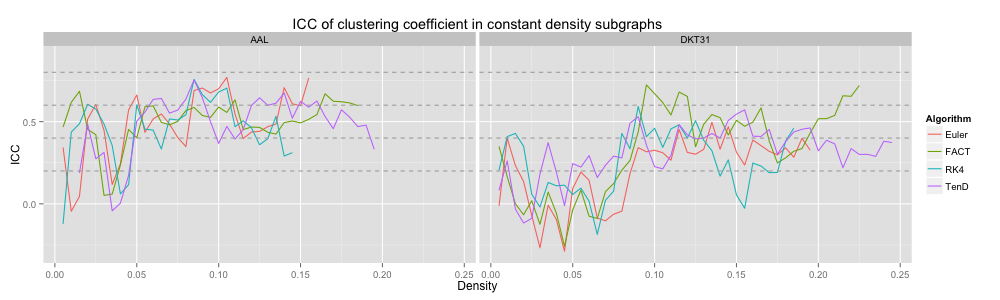
\includegraphics[width=\linewidth]{figures/clust_icc_plot.png}
\caption{Clust}
\label{fig:clust}
\end{center}
\end{figure*}

% FIXME - efficiency numbers are placeholders for now
\begin{table}[!t]
\processtable{Functional data analysis is used along with permutation
  testing to look for pair-wise differences in graph metrics resulting from different
  fiber tracking algorithms. Only the first time-point for each
  subject is used. For each metric, the upper-triangular values are for p-values for
  the AAL labels while the lower-triangular values were generated with
  the DKT31 labelset.\label{tab:permtesting}}
{\begin{tabular}{l | llll | llll }
\midrule
 & \multicolumn{4}{c}{Clustering Coefficient} &  \multicolumn{4}{c}{Characteristic Path Length} \\ \midrule
         & Euler    & FACT     & RK4        & TenD       & Euler    & FACT     & RK4        & TenD      \\\midrule
Euler  &            & 0.2511  & 0.6098    & 0.0374*   &            & 0.1646  & 0.3253    &  0.6984  \\
FACT & 0.6950 &              & 0.0256*  & 0.3175     & 0.9827 &            &  0.0063*   & 0.1662     \\
RK4   & 0.9866 & 0.7321  &               & 0.0050*   & 0.9180 & 0.5780  &                 & 0.1989   \\
TenD & 0.1343 & 0.8699  & 0.2010    &                & 0.8914 & 0.9285  & 0.8293   &    \\ \midrule
 & \multicolumn{4}{c}{Connected Component Size} &  \multicolumn{4}{c}{Graph Metric} \\ \midrule
Euler  &            & 0.3471  & 0.9324    & 0.7556   &            & 0.3506  & 0.1716   &  0.7984  \\
FACT & 0.9447 &              & 0.0468*  & 0.3025     & 0.5986 &            &  0.0344   & 0.296     \\
RK4   & 0.9998 &  0.7610  &              & 0.4748   & 0.4270 & 0.7780  &               & 0.3064   \\
TenD & 0.7912 & 0.8336  & 0.7269   &                & 0.9262 & 0.5958  & 0.4084   &    \\ \midrule
\end{tabular}}{}
 & \multicolumn{4}{c}{Global Efficiency} &  \multicolumn{4}{c}{Graph Metric} \\ \midrule
Euler  &            & 0.4657  & 0.3318    & 0.8574   &            & 0.3506  & 0.1716   &  0.7984  \\
FACT & 0.9869 &              & 0.0228*  & 0.5140     & 0.5986 &            &  0.0344   & 0.296     \\
RK4   & 0.9553 &  0.9050  &              & 0.3058   & 0.4270 & 0.7780  &               & 0.3064   \\
TenD & 0.5298 & 0.4753  & 0.8465    &                & 0.9262 & 0.5958  & 0.4084   &    \\ \midrule
\end{tabular}}{}
\end{table}


%\begin{table}[!t]
%\processtable{Resolution Requirements for the figures\label{Tab:01}}
%{\begin{tabular}{lllll}\toprule
%Image Type & Description & Format & Color Mode & Resolution\\\midrule
%Line Art & An image composed of lines and text,  & TIFF, EPS, JPEG & RGB, Bitmap & 900 - 1200 dpi\\
%          & which does not contain tonal or shaded areas.& & &\\
%         Halftone & A continuous tone photograph, which contains no text. & TIFF, EPS, JPEG & RGB, Grayscale & 300 dpi\\
%Combination & Image contains halftone + text or line art elements. & TIFF, EPS, JPEG & RGB,Grayscale & 600 - 900 dpi\\\botrule
%\end{tabular}}{This is a footnote}
%\end{table}

%\begin{equation}
%\sum x+ y =Z\label{eq:01}
%\end{equation}

%\textbf{Table\ref{Tab:01}} shows the resolution requirements for the figures. The figures must be legible:
%\begin{enumerate}
%\item The smallest visible text is no less than 8 points in height, when viewed at actual size.
%\item Solid lines are not broken up.
%\item Image areas are not pixelated or stair stepped.
%\item Text is legible and of high quality.
%\item Any lines in the graphic are no smaller than 2 points width.
%\end{enumerate}

%\textbf{Figure 2.}{ Enter the caption for your figure here.  Repeat as  necessary for each of your figures.}\label{fig:02}

\section{Discussion}
% Discussion: This section may be divided by subheadings. Discussions
% should cover the key findings of the study: discuss any prior art
% related to the subject so to place the novelty of the discovery in
% the appropriate context; discuss the potential short-comings and
% limitations on their interpretations; discuss their integration into
% the current understanding of the problem and how this advances the
% current views; speculate on the future direction of the research and
% freely postulate theories that could be tested in the future.


Other modalities, not examined here,
were also acquired making this data useful for future examinations of
structure and function.

No smoothing of data here

Other DTI scalar metrics, such as RD, or from other modalities such as MTR.

Did not normalize matrices

\subsection{Data Sharing}
%Frontiers supports the policy of data sharing, and authors are advised to make freely available any materials and information described in their article, and any data relevant to the article (while not compromising confidentiality in the context of human-subject research) that may be reasonably requested by others for the purpose of academic and non-commercial research. In regards to deposition of data and data sharing through databases, Frontiers urges authors to comply with the current best practices within their discipline.

\section*{Disclosure/Conflict-of-Interest Statement}
%All relationships financial, commercial or otherwise that might be perceived by the academic community as representing a potential conflict of interest must be described. If no such relationship exists, authors will be asked to declare that the research was conducted in the absence of any commercial or financial relationships that could be construed as a potential conflict of interest.
The authors declare that the research was conducted in the absence of any commercial or financial relationships that could be construed as a potential conflict of interest.

\section*{Acknowledgement}
Shoutouts to our peeps

\paragraph{Funding\textcolon} Shoutout to our peep\$

\section*{Supplemental Data}
Maybe need this, maybe not

\bibliographystyle{frontiersinSCNS} % for Science articles
%\bibliographystyle{frontiersinMED} % for Medicine articles
\bibliography{priorwork}

%\begin{thebibliography}{}

%\bibitem[Bofelli {et~al}., 2000]{Boffelli03} Bofelli,F., Name2, Name3 (2003) Article title, {\it Journal Name}, 199, 133-154.

%\bibitem[Bag {et~al}., 2001]{Bag01} Bag,M., Name2, Name3 (2001) Article title, {\it Journal Name}, 99, 33-54.

%\end{thebibliography}
\end{document}
